\chapter{Diagramme de Gantt}

Le diagramme de Gantt, montré à la figure \ref{fig:Gantt} est un outil qui permet de visulaliser l'ensemble du projet au fil du temps.
On y retrouve les tâches essentielles au bon fonctionnement du projet ainsi que les plages de temps prévues pour chacunes.
Les tâches sont également reliées entre elles, puisque certaines parties du projet ne peuvent être accomplies que si d'autres sont terminées.
Par exemple, il est plus facile de détecter la station de recharge après l'avoir construite.

\begin{figure}[ht]
    \centering
    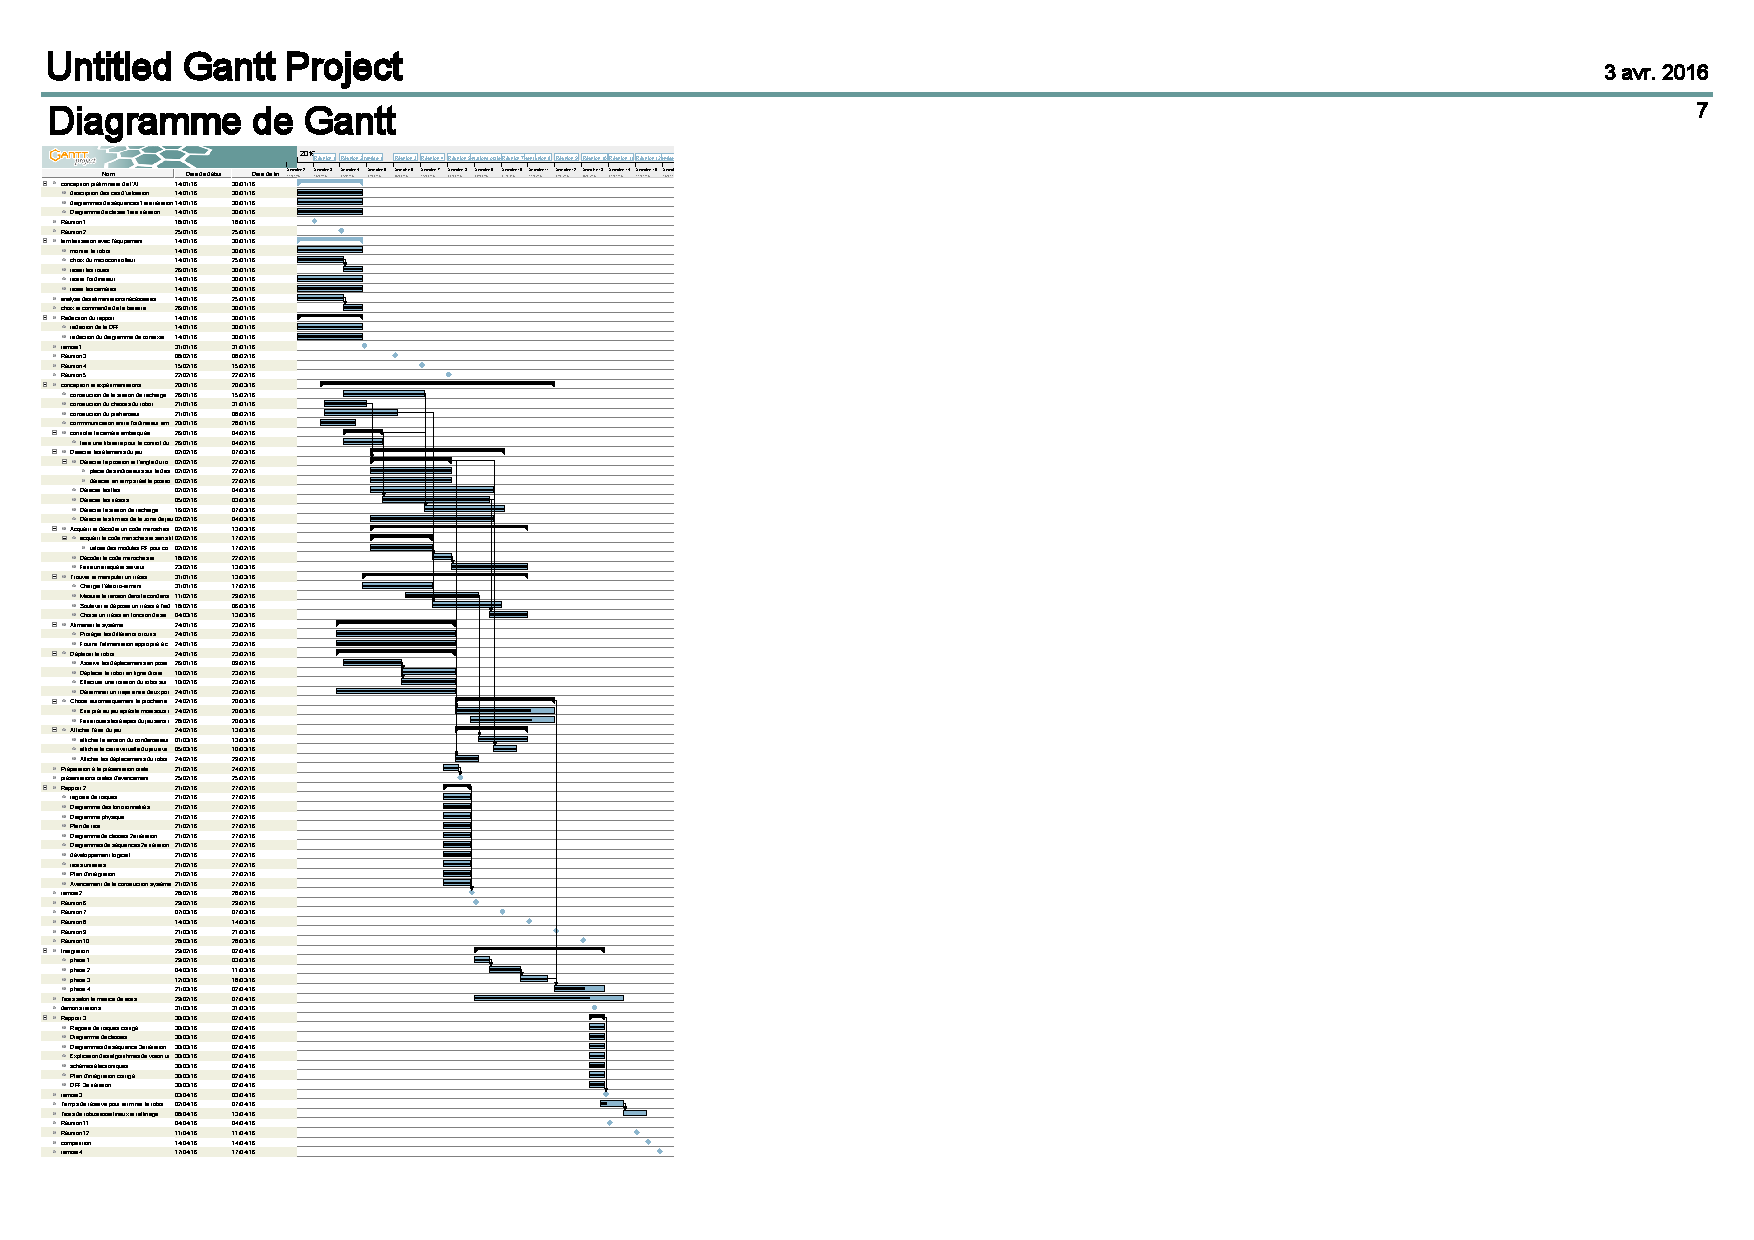
\includegraphics[scale=1, trim = 0 0 16cm 2.5cm, clip]{resources/gantt.pdf}
    \caption{Diagramme de Gantt}
    \label{fig:Gantt}
  \end{figure}
